\section{Benchmark Problems}

In this section several benchmark problems are introduced illustrating the capabilities of PFLOTRAN.

\subsection{Ion Exchange}

Voegelin et al. (2000) present results of ion exchange in a soil column for the system Ca-Mg-Na. Here PFLOTRAN is applied to this problem using the Gaines-Thomas exchange model. Soil column C1 with length 48.1 cm and diameter 0.3 cm was used for the simulations. A flow rate of 5.6 cm/min was used in the experiment. The inlet solution was changed during the coarse of the experiment at 20 and 65 pore volumes with cation compositions listed in Table 2 of Voegelin et al. (2000). The CEC of the soil used in the experiments was determined to have a value of 0.06$\pm$0.002 mol/kg. As PFLOTRAN requires the CEC in units of mol/m$^3$ this was obtained from the formula
\begin{subequations}
\BA
\omega &\eq \frac{N_s}{V} \eq \frac{N_s}{M_s} \frac{M_s}{V_s}\frac{V_s}{V},\\\
&\eq \rho_s (1-\varphi) {\rm CEC}.
\EA
\end{subequations}
Using a porosity of 0.61 and solid grain density of 3.0344 g/cm$^3$, yielded $\omega = 71.004$ mol/m$^3$. The results of the simulation are shown in Figure~\ref{fionex} along with data reported by Voegelin et al. (2000). Self-sharpening fronts can be observed at approximately 10 and 71 at pore volumes, and a self-broadening front from 30-55 pore volumes where agreement with experiment is not as good.

The input file for the simulation is listed in Table~\ref{tionex}.

\begin{figure}[h]\centering
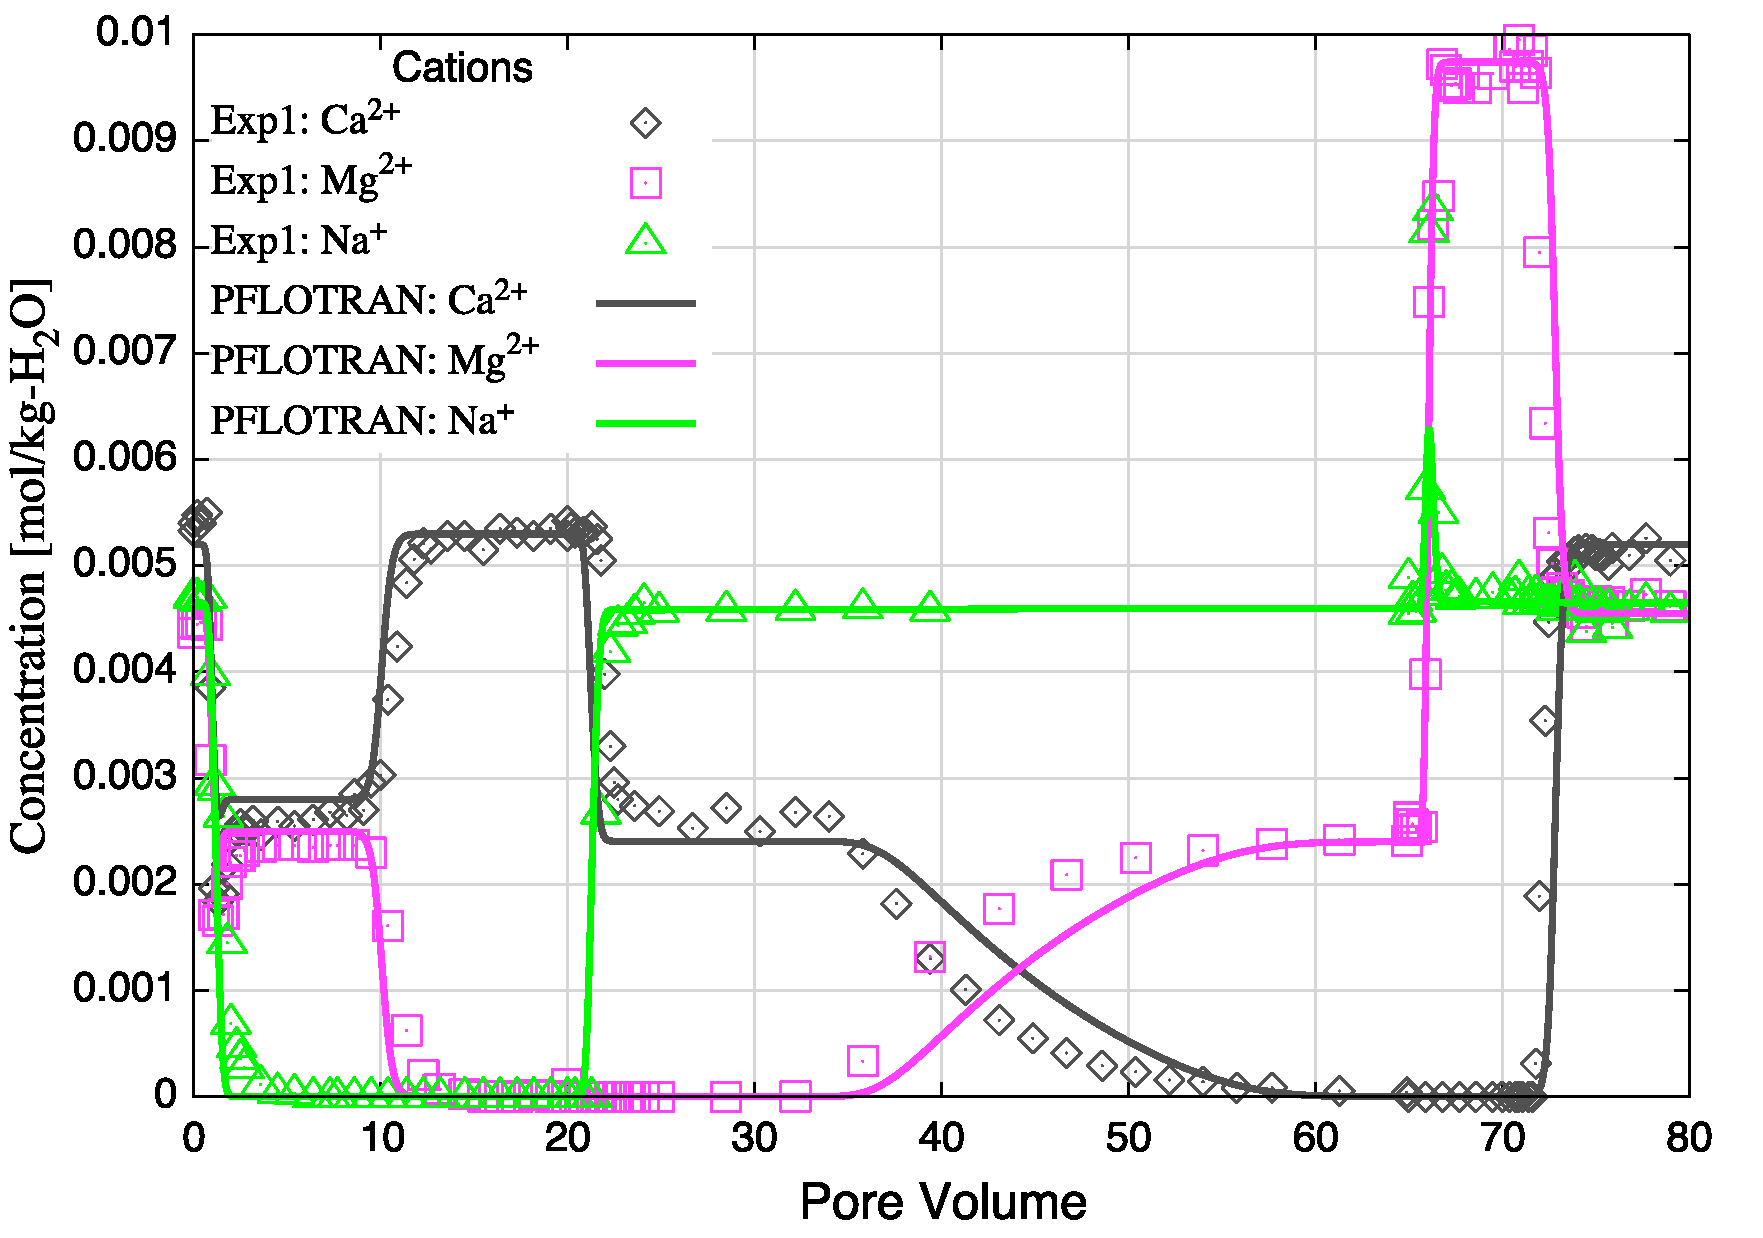
\includegraphics[scale=0.5]{./figs/ionex}
\caption{Breakthrough curves for Ca$^{2+}$, Mg$^{2+}$ and Na$^+$ compared with experimental results from Voegelin et al. (2000).}\label{fionex}
\end{figure}

\newpage
%\footnotesize
\scriptsize
\VerbatimInput{./inputfiles/ionex.in}\label{tionex}
\normalsize

\newpage

\subsection{GENERAL\_REACTION Example}

\subsubsection{Problem Description}

%\subsubsection{Governing Equations}

A single irreversible reaction is considered of the form
\EQ
A + 2 B \rightarrow C,
\EN
for flow in a fully saturated 1D column of length 100 m with a Darcy velocity of 1 m/y, diffusion coefficient of $10^{-9}$ m$^2$/s and porosity equal to 0.25.
The conservation equation for advection, diffusion and reaction is given by
\EQ
\frac{\p}{\p t} \varphi C_l + \bnabla\cdot\bF_l \eq - \varphi \nu_l \R, \ \ \ \ (l=A,\,B,\,C), 
\EN
with stoichiometric coefficients $\nu_A = 1$, $\nu_B = 2$, and $\nu_C=-1$.
The flux $\bF_l$ consists of contributions from advection and diffusion
\EQ
\bF_l \eq \bq C_l - \varphi D \bnabla C_l.
\EN
The forward reaction rate is based on a elementary aqueous reaction
\EQ
\R \eq k_f C_A^{\nu_A} C_B^{\nu_B}.
\EN
%\BA
%\frac{\p\R}{\p C_{l}} \eq \frac{\nu_l}{C_{l}} \R
%\EA
Dividing through by porosity (assuming $\varphi$ = constant), the transport equation becomes
\EQ
\frac{\p C_l}{\p t} + \bnabla\cdot\bv C_l - D \bnabla\cdot\bnabla C_l + \nu_l^{} k_{\!f}^{} C_A^{\nu_A} C_B^{\nu_B} \eq 0,
\EN
with average pore velocity 
\EQ
\bv \eq \frac{\bq}{\varphi}.
\EN
Initial and boundary conditions imposed on the solution are given by
\begin{subequations}
\BA
C(x,t=0) &\eq C_\infty,\\
C(x=0,\,t) &\eq C_0,\\
\left.\frac{\p C}{\p x} \right|_{x=l_x} &\eq 0.
%\left.\frac{\p C}{\p y} \right|_{y=0,\,y=l_y} &\eq 0.
\EA
\end{subequations}

\subsubsection{Simulation Results}

Results are shown in Figure~\ref{fabc} for the concentrations of species A, B, C at 5 years obtained from PFLOTRAN and a prototype code written in C++ based on the PETSc TS time stepping class. The code uses a backward Euler (TSBEULER) time integrator with nodes placed at the grid cell corners. The slight discrepancy between the results of the two codes may be due to the use of a finite volume cell-centered grid in PFLOTRAN, versus the corner-node grid used in the prototype code.

\begin{figure}[h]\centering
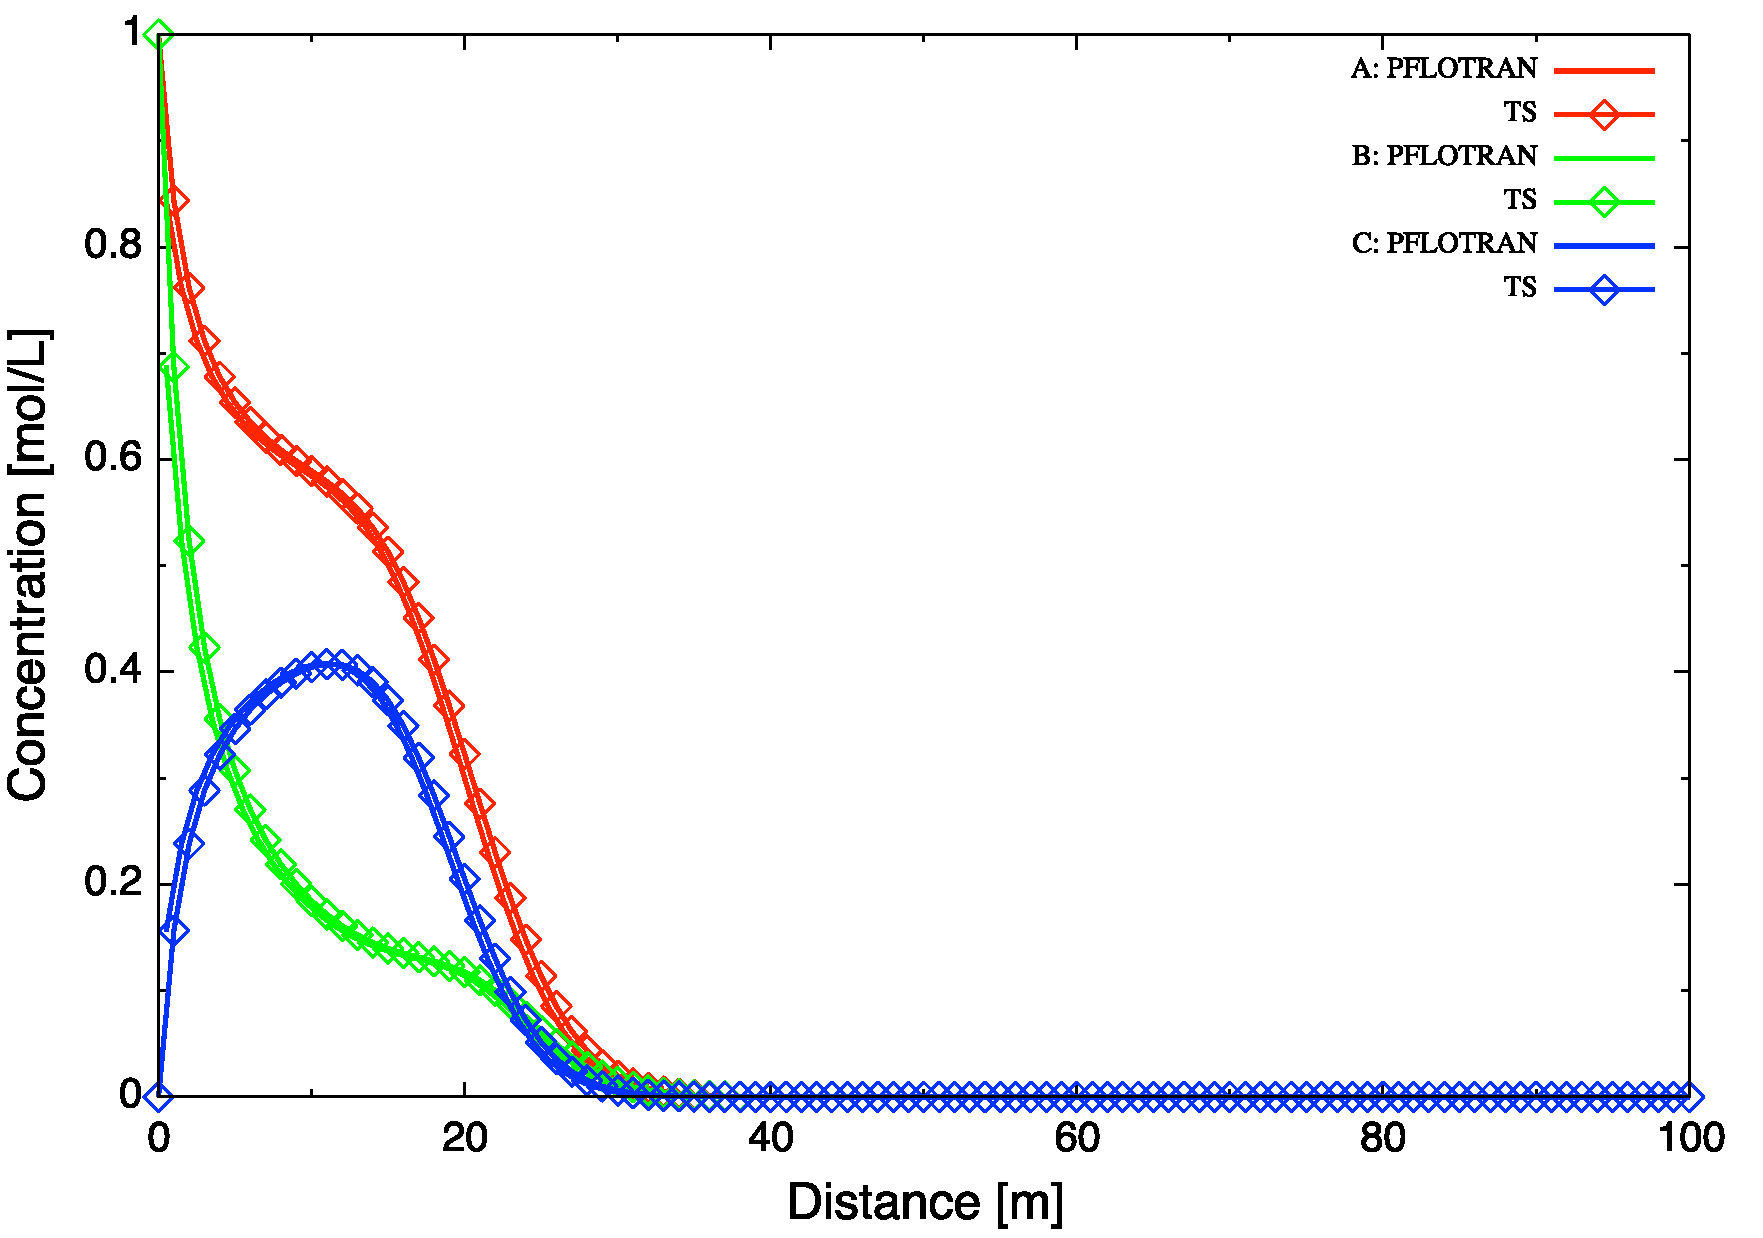
\includegraphics[scale=0.5]{./figs/abc}
\caption{Comparison of concentrations for species A, B, C plotted as a function of distance for an elapsed time of 5 years for PFLOTRAN and a prototype code based on PETSc's TS class.}\label{fabc}
\end{figure}

\subsubsection{PFLOTRAN Input File}

%\footnotesize
\scriptsize
\VerbatimInput{./inputfiles/ABC/ABC1d.in}\label{tabc}
\normalsize

\newpage

\subsection{RICHARDS Mode with Tracer: SX-115 Hanford Tank Farm}

\subsubsection{Problem Description}

The saturation profile is computed for both steady-state and transient conditions in a 1D vertical column consisting of a layered porous medium representing the Hanford sediment in the vicinity of the S/SX tank farm. The transient case simulates a leak from the base of the SX-115 tank. This problem description is taken from Lichtner et al. (2004).

\subsubsection{Governing Equations}

The moisture profile is calculated using parameters related to the Hanford sediment at the S/SX tank farm based on the Richards equation for variably saturated porous media. The Hanford sediment is composed of five layers with the properties listed in Tables~\ref{t1} and \ref{t2}. The governing equations consist of Richards equation for variably saturated fluid flow given by
\EQ
\frac{\p}{\p t} \varphi s\rho + \bnabla\cdot\bq\rho \eq Q,
\EN
and solute transport of a tracer
\EQ
\frac{\p}{\p t}\varphi C + \bnabla\cdot\big(\bq C - \varphi s \tau D \bnabla C\big) \eq Q_C.
\EN
In these equations $\varphi$ denotes the spatially variable porosity of the porous medium assumed to constant within each stratigraphic layer, $s$ gives the saturation state of the porous medium, $\rho$ represents the fluid density in general a function of pressure and temperature, $C$ denotes the solute concentration, $D$ denotes the diffusion/dispersion coefficient, $\tau$ represents tortuosity, $Q$ and $Q_C$ denote source/sink terms, and $\bq$ denotes the Darcy velocity defined by
\EQ
\bq\eq - \frac{k_{\rm sat}k_r}{\mu} \bnabla (p-\rho g z),
\EN
with saturated permeability $k_{\rm sat}$, relative permeability $k_r$, fluid viscosity $\mu$, pressure $p$, formula weight of water $W$, acceleration of gravity $g$, and height $z$. Van Genuchten capillary properties are used for relative relative permeability according to the relation
\EQ\label{kr}
k_{r} \eq \sqrt{s_{\rm eff}} \left\{1 - \left[1- \left( s_l^{\rm 
eff} \right)^{1/m} \right]^m \right\}^2, 
\EN
where $s_{\rm eff}$ is related to capillary pressure $P_c$ by the equation
\EQ\label{sat}
s_{\rm eff} \eq \left[1+\left( \alpha |P_c| \right)^n 
\right]^{-m}, 
\EN 
where $s_{\rm 
eff}$ is defined by 
\EQ\label{seff1}
s_{\rm eff} \eq \frac{s - s_r}{1 - s_r}, 
\EN 
and where $s_r$ denotes the residual saturation. The quantity $n$ is related to $m$ by the expression 
\EQ\label{lambda} 
m \eq 1-\frac{1}{n}, \ \ \ \ \ n \eq \frac{1}{1-m}. 
\EN 
The capillary pressure $P_c$ and fluid pressure $p$ are related by the (constant) gas pressure $p_g^0$
\EQ
P_c \eq p_g^0-p,
\EN
where $p_g^0 \!=\! 101,325$ Pa is set to atmospheric pressure.

\paragraph{Semi-Analytical Solution for Steady-State Conditions}

For steady-state conditions the saturation profile satisfies the equation
\EQ
\frac{d}{dz} \rho q_z \eq 0,
\EN
or assuming an incompressible fluid
\EQ
q_z \eq q_z^0,
\EN
where $q_z^0$ denotes infiltration at the surface. Thus the pressure is obtained as a function of $z$ by solving the ODE
\EQ\label{dpdz}
\frac{dp}{dz} \eq -\frac{\mu q_z^0}{k_{\rm sat} k_r} - \rho g,
\EN
using Eqns.\eqref{kr} and \eqref{sat} to express the relative permeability $k_r$ as a function of pressure. For the special case of zero infiltration it follows that
\EQ
p(z) \eq p_0 - \rho g (z-z_0),
\EN
with $p(z_0)\!=\!p_0$. The saturation profile is obtained from Eqns.\eqref{sat} and \eqref{seff}.

\paragraph{Watertable}

The position of the watertable is defined by vanishing of the capillary pressure
\EQ
P_c(z_{\rm wt}) \eq 0,
\EN
where $z_{\rm wt}$ denotes the height of the watertable. For the case with no infiltration at the surface it follows that
\EQ
z_{\rm wt} \eq z_0 + \frac{p_0-p_g}{\rho g},
\EN
with the boundary condition $p(z_0) = p_0$ and $z_0$ denotes the datum. If $p_0$ is set equal to $p_g$, then $z_{\rm wt} = z_0$, or the height of the watertable is equal to the datum.
The same holds true also with constant nonzero infiltration. 

\begin{comment}
To see this note that the pressure satisfies Eqn.\eqref{dpdz}. Integrating this equation yields
\EQ
p(z) \eq p_0 - \rho g (z-z_0) -\frac{\mu q_z^0}{k_{\rm sat}} \int_{z_0}^z \frac{dz'}{k_r}.
\EN
Thus the watertable is determined implicitly from the equation
\EQ\label{wt}
z_{\rm wt} \eq z_0 + \frac{p_0 -p_g}{\rho g} + \frac{\mu q_z^0}{\rho g k_{\rm sat}} \int_{z_0}^{z_{\rm wt}} \frac{dz}{k_r}.
\EN
Note that if $z_{\rm wt} = z_0$, the integral on the right-hand side vanishes.
Expanding the integral on the right-hand side yields
\BA
\int_{z_0}^{z_{\rm wt}} \F dz' &\eq \frac{\G_0}{\rho g} \int_{z_0}^{z_{\rm wt}} \Big[\F_0 + \frac{1}{1!}\F_0' z' + \frac{1}{2!} \F_0'' (z')^2 + \cdots \Big] dz',\\
&\eq \frac{\G_0}{\rho g} \Big[\F_0 (z_{\rm wt}-z_0) + \frac{1}{1! 2}\F_0' (z_{\rm wt}^2-z_0^2) + \frac{1}{2! 3} \F_0'' (z_{\rm wt}^3-z_0^3) + \cdots  \Big].
\EA
Consequently, it is clear that for $p_0=p_g$, $z_{\rm wt}=z_0$ satisfies Eqn.\eqref{wt}. For $p_0\ne p_g$, the watertable height depends on $q_z^0$.
\end{comment}

\subsubsection{Model Parameters}

Model parameters used in the simulations are listed in Tables~\ref{t1} and \ref{t2}. Although not needed here, thermal properties are also listed. Diffusivity was set to $10^{-9}$ m$^2$ s$^{-1}$ and tortuosity was set to one.

\renewcommand{\tabcolsep}{1.7mm}

\begin{table}[H]\centering
\caption{Stratigraphic sequence used in the calculations, after Ward et al. (1996).}\label{t1}

\vspace{3mm}

\begin{tabular}{lcr}
\toprule
Formation & Abbrev. & Thickness [m]\\
\midrule
Backfill & BF & 16.0\\
Hanford Fine Sand & HF & 23.0\\
Plio-Pleistocene & PP & 6.0\\
Upper Ringold Gravel & URG & 3.0\\
Middle Ringold Gravel & MRG & 20.0\\
\bottomrule
\end{tabular}
\end{table}

\begin{table}[H]\centering
\caption{Parameters for material and thermal properties for intrinsic rock density $\rho_s$, heat capacity $c$, thermal conductivity $\kappa$, porosity $\varphi$, residual water saturation $s_r$, van Genuchten parameters $\alpha$ and $\lambda$, and vertical water saturated permeability $k_{\rm sat}$. Data taken from Khaleel and Freeman (1995), Khaleel et al. (2001), and Pruess et al. (2002).}\label{t2}

\vspace{3mm}

\begin{tabular}{lccccccccc}
\toprule
Formation & $\rho_s$ & $c$ & $\kappa_{\rm dry}$ & $\kappa_{\rm wet}$ & $\varphi$ & $s_r$ & $\alpha$ & $m$ & $k_{\rm sat}$\\
& g cm$^{-3}$ & J kg$^{-1}$ K$^{-1}$ & \multicolumn{2}{c}{W m$^{-1}$} & --- & --- & Pa$^{-1}$ & --- & m$^2$\\
\midrule
BF  & 2.8 & 800 & 0.5 & 2 & 0.2585 & 0.0774 & 1.008e-3 & 0.6585  &1.240e-12\\
HF  & 2.8 & 800 & 0.5 & 2 & 0.3586 & 0.0837 & 9.408e-5 & 0.4694  &3.370e-13\\
PP  & 2.8 & 800 & 0.5 & 2 & 0.4223 & 0.2595 & 6.851e-5 & 0.4559  &3.735e-14\\
URG & 2.8 & 800 & 0.5 & 2 & 0.2625 & 0.2130 & 2.966e-5 & 0.3859  &1.439e-13\\
MRG & 2.8 & 800 & 0.5 & 2 & 0.1643 & 0.0609 & 6.340e-5 & 0.3922  &2.004e-13\\
\bottomrule
\end{tabular}
\end{table}

\subsubsection{Simulation Results}

The calculations are carried out for an isothermal system using Richards equation. First, the steady-state saturation profile is obtained without the tank leak present. Then using the steady-state profile as the initial condition the tank leak is turned on. The results for the steady-state saturation and pressure profiles are shown in Figure~\ref{f1} for infiltration rates at the surface of 0, 8 and 80 mm/y. The mean infiltration rate at the Hanford site is approximately 8 mm/y. A 1D column 68 m heigh with the water table located at a height of 6 m from the bottom is used in the simulation. A uniform grid spacing of 0.5 m is used to discretize Richards equation.

Shown in Figure~\ref{f2} is the saturation at different times following a two week leak releasing 60,000 gallons from the SX-115 tank at a depth of 16 m. In the simulation a release rate of $1.87\!\times\! 10^{-3}$ kg/s is used.


\clearpage

\begin{figure}[h]\centering
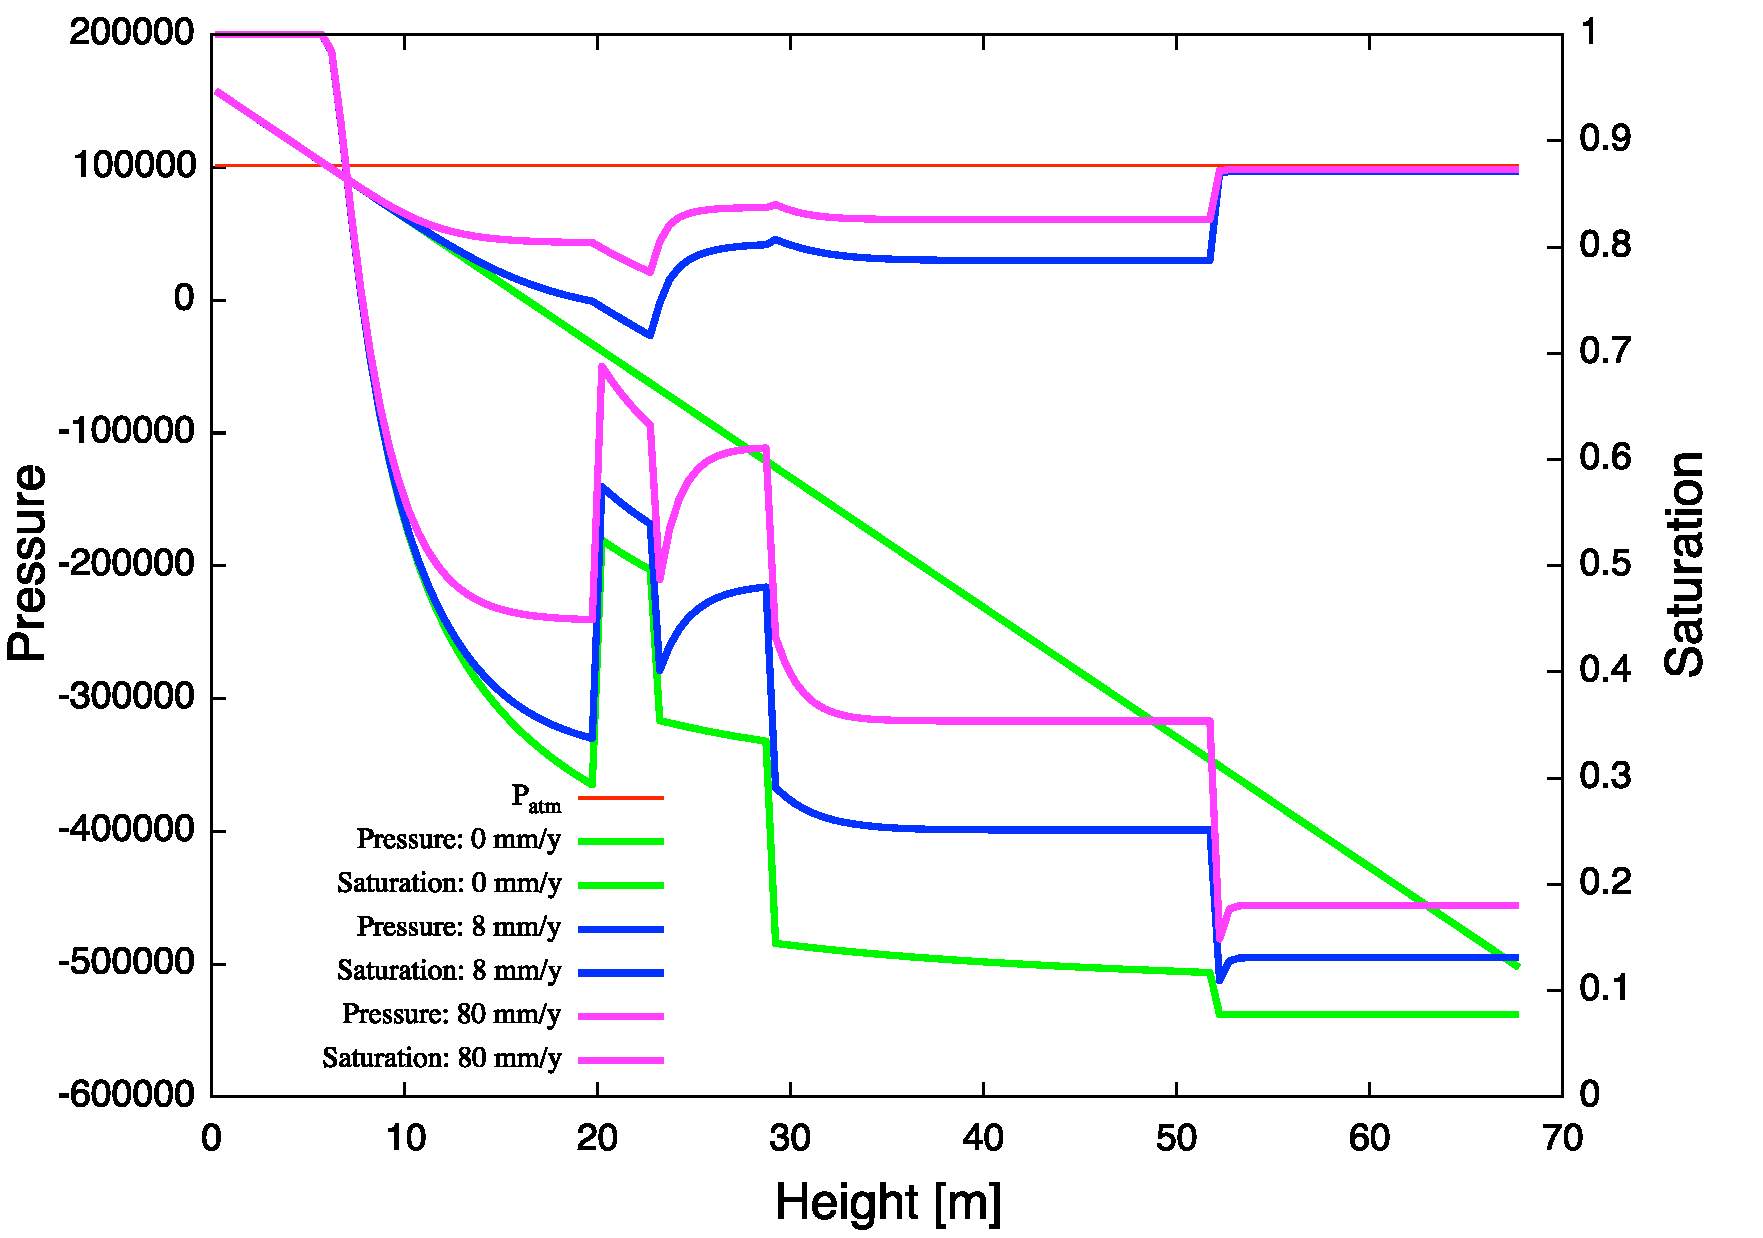
\includegraphics[scale=0.45]{./figs/ps}
\caption{Steady-state saturation and pressure profiles for infiltration rates of 0, 8 and 80 mm/y. The water table is located at 6 m from the bottom of the computational domain.}\label{f1}
\end{figure}

\begin{figure}[h]\centering
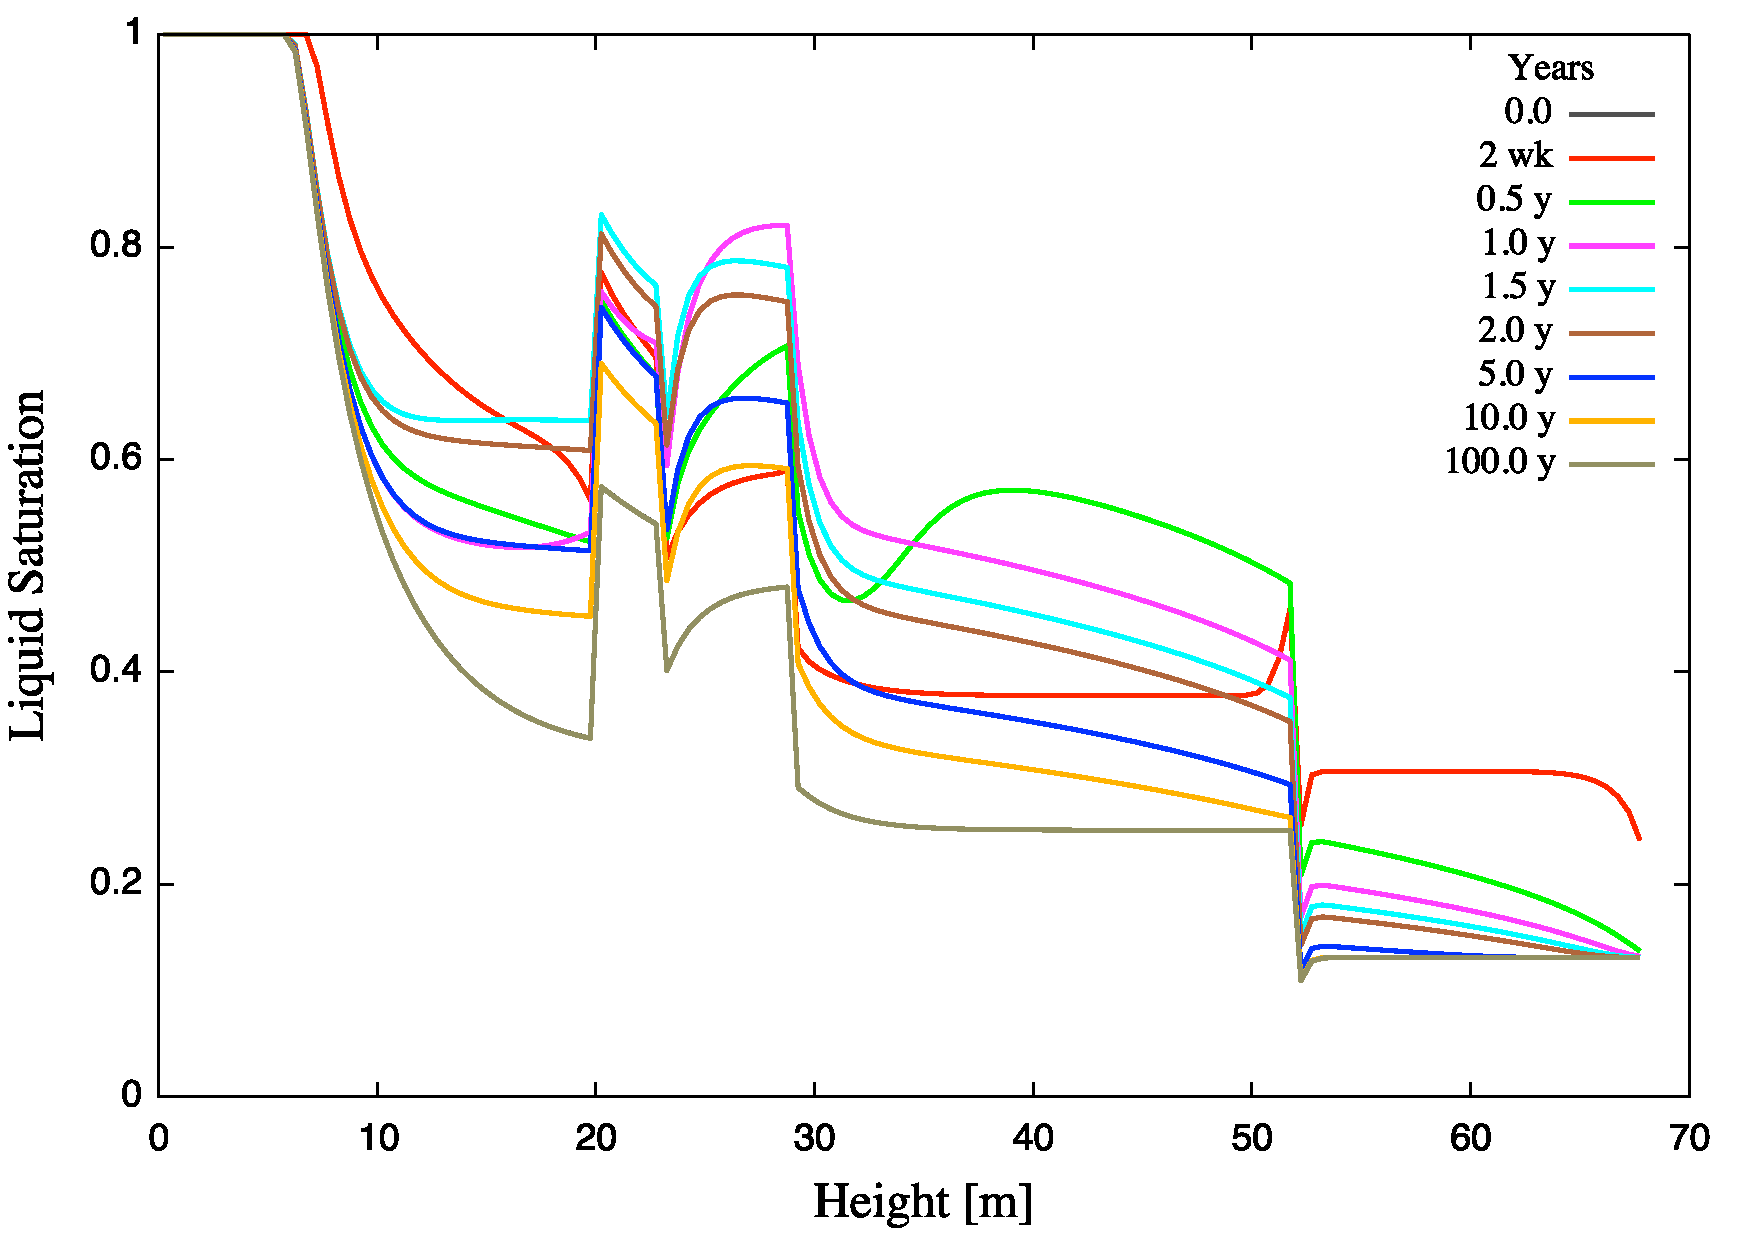
\includegraphics[scale=0.45]{./figs/sat_leak}
\caption{Simulation of a tank leak with a duration of two weeks showing the saturation profile for different times indicated in the figure.}\label{f2}
\end{figure}

\begin{figure}[h]\centering
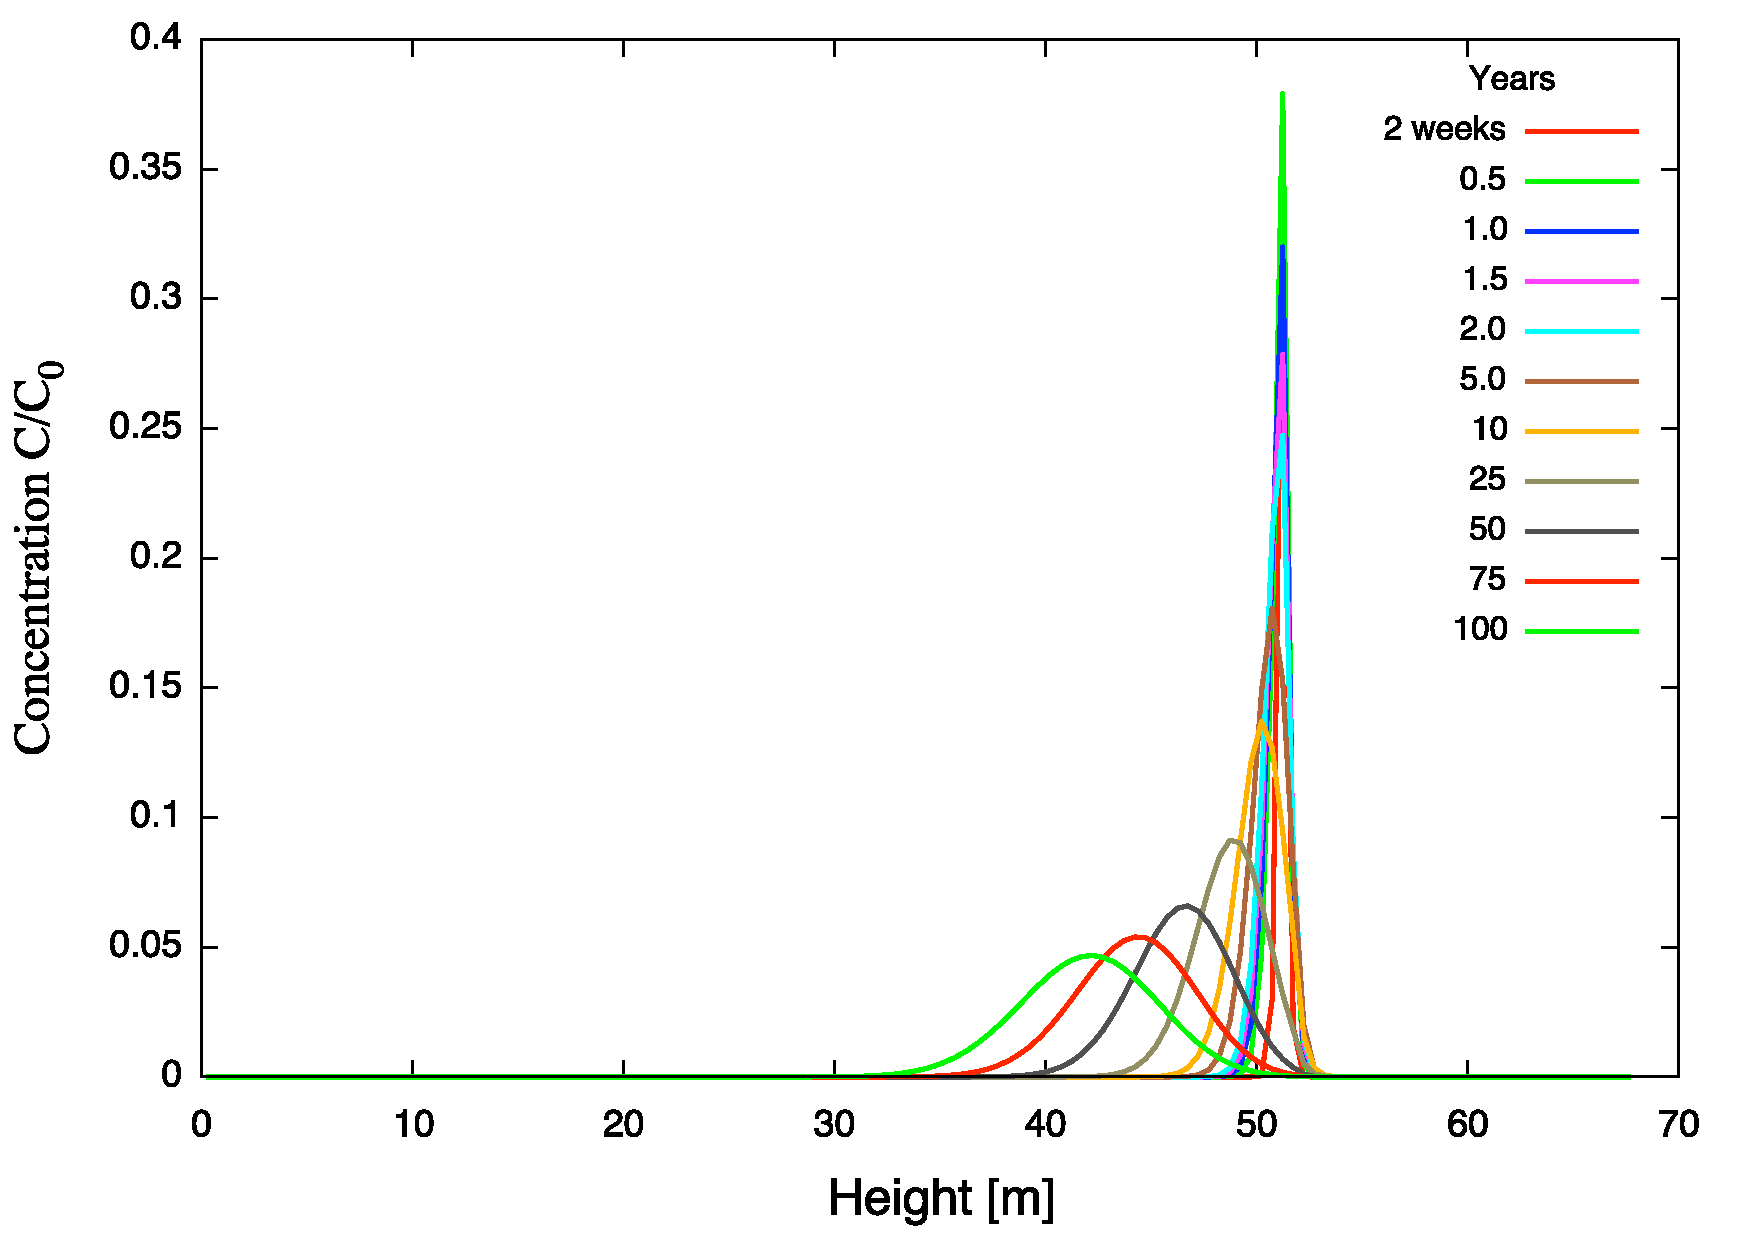
\includegraphics[scale=0.45]{./figs/conc}
\caption{The solute concentration profile corresponding to Figure~\ref{t2} for different times indicated in the figure.}\label{f3}
\end{figure}

\clearpage

\subsubsection{PFLOTRAN Input File}

Listing for the PFLOTRAN input file coupling Richards mode to a tracer is given below. Note that the stratigraphic zone specification in {\tt REGION} is grid independent as is the grid size specification in keyword {\tt GRID}. Therefore to change the grid spacing only the line: {\tt NXYZ 1 1 136}, needs to be changed. Also note that lines beginning with \# are read as a comment as is input following `!'.

\bigskip

\noindent PFLOTRAN input file {\tt pflotran.in}: 
%\footnotesize
\scriptsize

\VerbatimInput{./inputfiles/sx115/sx115.in}

\clearpage

\normalsize
\noindent
Source/sink file {\tt src.dat}:
%\footnotesize
\scriptsize
\VerbatimInput{./inputfiles/sx115/src.dat}
\normalsize

\subsection{MPHASE}

\subsubsection{CO$_2$ Sequestration: 1D Example Problem and Comparison with\\ TOUGHREACT}

In this example problem involves sequentially coupling of {\tt MPHASE} and {\tt CHEMISTRY}. The chemical system consists of four primary species and 5 secondary species. Supercritical CO$_2$ is injected into a well located at the west boundary. Dirichlet pressure boundary conditions are imposed at the east boundary. The problem definition with associated parameters is given in Table~\ref{tco2}.

\begin{table}[h]\centering
\caption{Problem definition and parameters used in the 1D CO$_2$ sequestration example.}
\label{tco2}
\vspace{3mm}
\begin{tabular}{lcc}
\toprule
Description & Symbol & Value\\
\midrule
Domain & $l$ & 100 m\\
Permeability & $k$ & $10^{-15}$ m$^2$\\
Porosity & $\varphi$ & 0.12\\
Tortuosity & $\tau$ & 1\\
Injection Rate & $Q_\c$ & $5\times 10^{-5}$ kg/s, duration 0.4 y\\
Characteristic Curves & modified van Genuchten & [see Eqns.\eqref{pc}-\eqref{sg}]\\
& $\lambda$ & 0.6\\
& $\a$ & $1.9 \times 10^{-5}$ Pa$^{-1}$\\
& $s_{rl}$ & 0\\
& $s_{rg}$ & 0\\
& $P_c^{\rm max}$ & $10^7$ Pa\\
Rock Density & $\rho_r$ & 2650 kg/m$^3$\\
Rock Specific Heat & $c_r$ & 1000 J/kg/K\\
Rock Thermal Conductivity & $\kappa_{\rm wet,\,dry}$ & 0.5 W/m/K\\
\bottomrule
\end{tabular}
\end{table}

The PFLOTRAN initial aqueous solution corresponds to a brine with NaCl concentration of 0.5 m. Mineral reactions are not considered. The initial fluid composition taken from {\tt pflotran.out} is listed in Table~\ref{tinitial_co2}.

\begin{table}[h]
\caption{Initial concentration of primary and secondary species. Mineral reactions are not considered.}
\label{tinitial_co2}
%\footnotesize
\scriptsize
\begin{verbatim}
  Transport Condition: Initial
  ----------------------------------------------------------------------------
        iterations:    20
                pH:   5.0273
    ionic strength:   4.7915E-01 [mol/L]
    charge balance:   1.1102E-16
          pressure:   1.6450E+07 [Pa]
       temperature:    54.50 [C]
       density H2O:   992.99 [kg/m^3]
 ln / activity H2O:   0.0000E+00  1.0000E+00    [---]
 mole fraction H2O:   9.8093E-01    [---]
 mass fraction H2O:   9.7160E-01    [---]
  ----------------------------------------------------------------------------
  primary               free        total
  species               molal       molal       act coef     constraint
  ----------------------------------------------------------------------------
  H+                    1.1727E-05  2.5844E-17  8.0079E-01    chrg
  Na+                   4.7913E-01  5.0000E-01  6.8288E-01    total aq
  Cl-                   4.7913E-01  5.0000E-01  6.4459E-01    total aq
  CO2(aq)               1.1380E-04  1.2551E-04  1.1053E+00    CO2(g)

  complex               molality    act coef  logK
  ----------------------------------------------------------------------------
  NaCl(aq)              2.0866E-02  1.0000E+00    6.8511E-01
  HCO3-                 1.1713E-05  6.8288E-01    6.2239E+00
  OH-                   1.2056E-08  6.6467E-01    1.3123E+01
  NaOH(aq)              1.6487E-09  1.0000E+00    1.3325E+01
  CO3--                 3.2433E-10  2.0899E-01    1.6323E+01
\end{verbatim}
\end{table}

\normalsize

The defining equations for the saturation and relative permeability functions for the aqueous solution and supercritical CO$_2$ are given by the van Genuchten -Corey relations. For the aqueous solution van Genuchten curves are used for capillary pressure $P_c$
\EQ\label{pc}
P_c(s_e) \eq \frac{1}{\a}\Big[\big(s_e\big)^{-1/\lambda} -1\big]^{1-\lambda},
\EN
and relative permeability $k_{rl}$
\EQ
k_{rl} \eq \sqrt{s_e}\left\{1-\left[1-\big( s_e \big)^{1/\lambda}\right]^\lambda\right\}^2,
\EN
with effective saturation $s_e$ defined by
\EQ
s_e \eq \frac{s_l - s_{lr}}{1-s_{lr}}.
\EN
For the supercritical CO$_2$ phase the Corey curve is used defined by
\EQ
k_{rg} \eq \big(1-s'\big)^2 \big[1-(s')^2\big],
\EN
with
\EQ\label{sg}
s' \eq \frac{s_l-s_{lr}}{1-s_{lr}-s_{gr}}.
\EN

Shown in Figure~\ref{fco2} is a comparison of PFLOTRAN with TOUGHREACT (TOUGHREACT results provided by Alt-Epping and Wanner, private comm.). The same thermodynamic database is used for both codes. Only slight differences can be seen. The CO$_2$ aqueous and total concentrations are essentially identical for PFLOTRAN in the low pH region where supercritical CO$_2$ is present, with slight differences for TOUGHREACT. Note that the CO$_2$ aqueous concentration (and mole fraction $X_{\rm CO_2}$ although not visible in the figure) obtained from PFLOTRAN is not exactly constant. This is caused, presumably, by a change in pressure as 
shown in Figure~\ref{fp} for the liquid and CO$_2$ pressures in addition to the CO$_2$ saturation $s_{\rm CO_2}$.

\begin{figure}[h]\centering
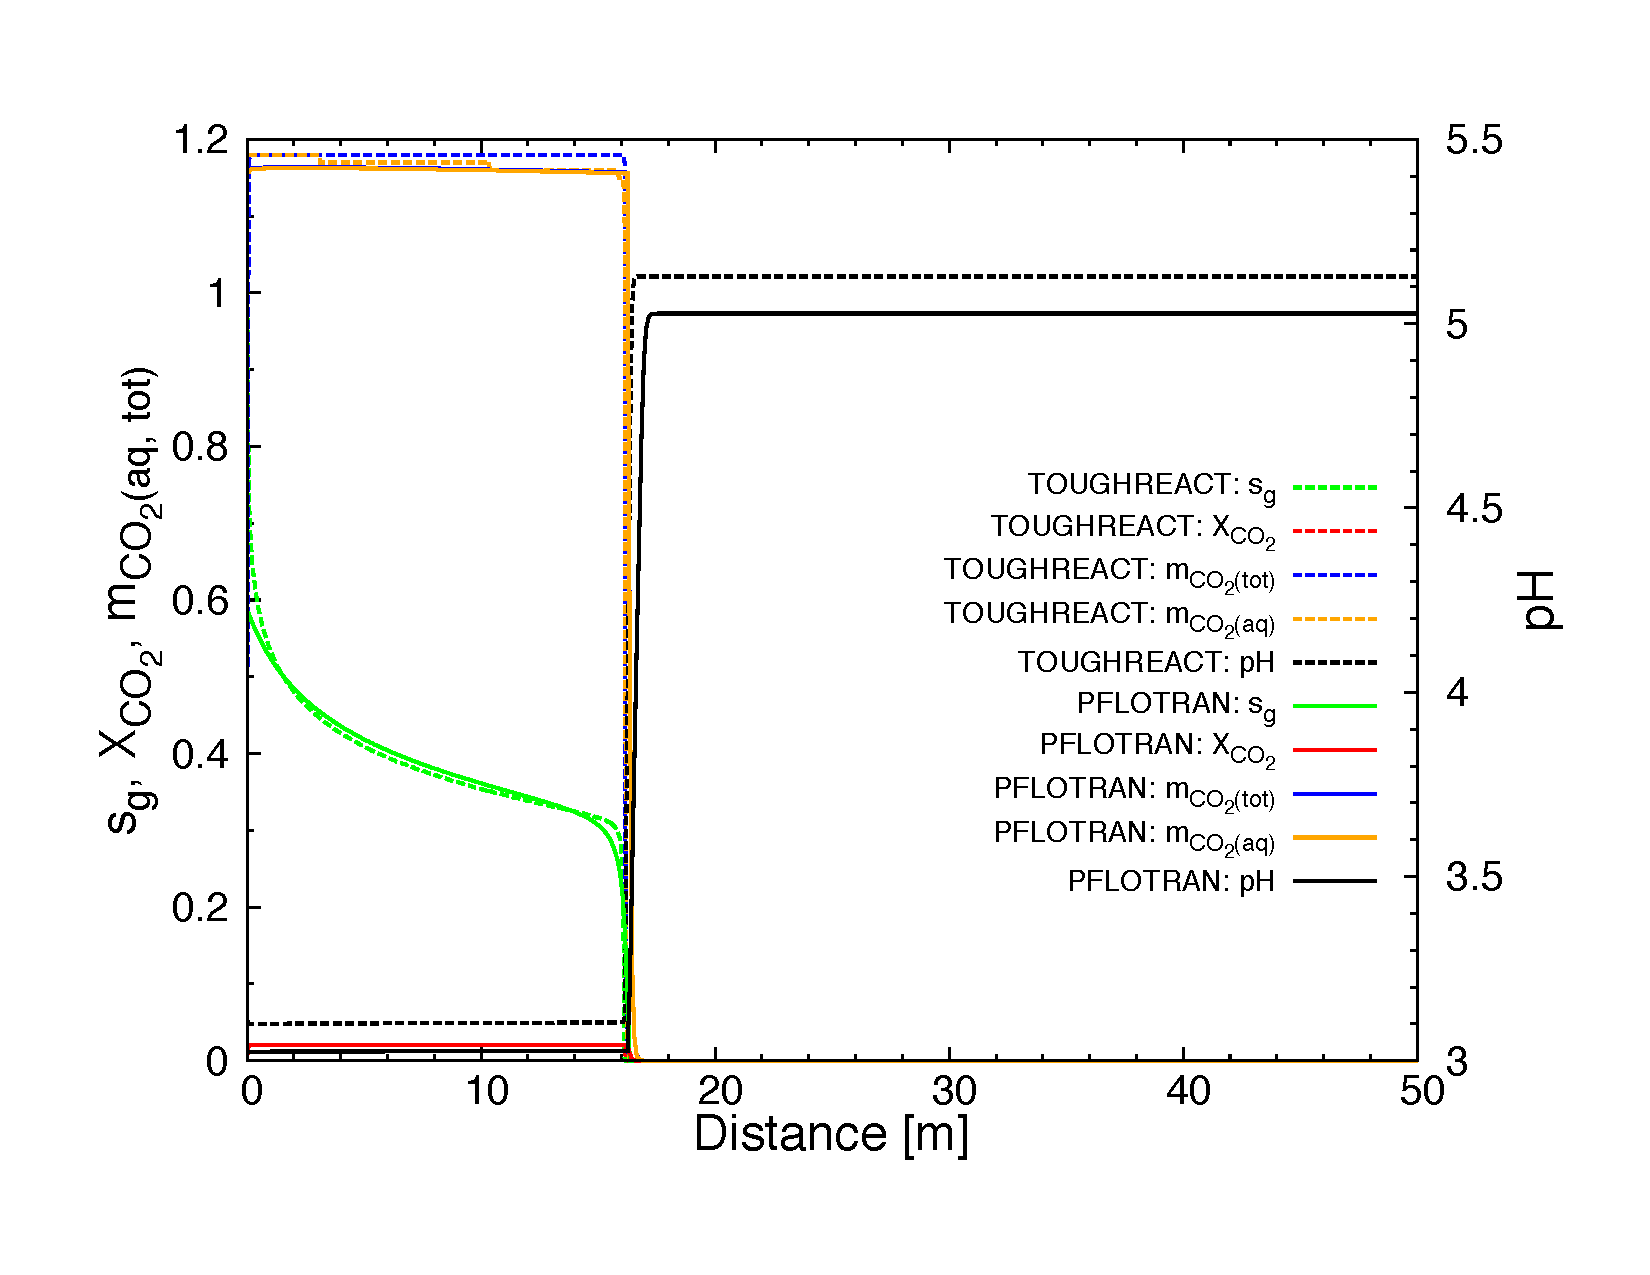
\includegraphics[width=\textwidth]{./figs/tr-pflotran-brine}

\vspace{-1.cm}

\parbox{5in}{
\caption{Comparison with TOUGHREACT (dashed curves) and PFLOTRAN (solid curves) after an elapsed time of 0.4 y corresponding to the end of injection. Reasonable agreement is obtained between the two codes.}
\label{fco2}}
\end{figure}

\begin{figure}[t]\centering
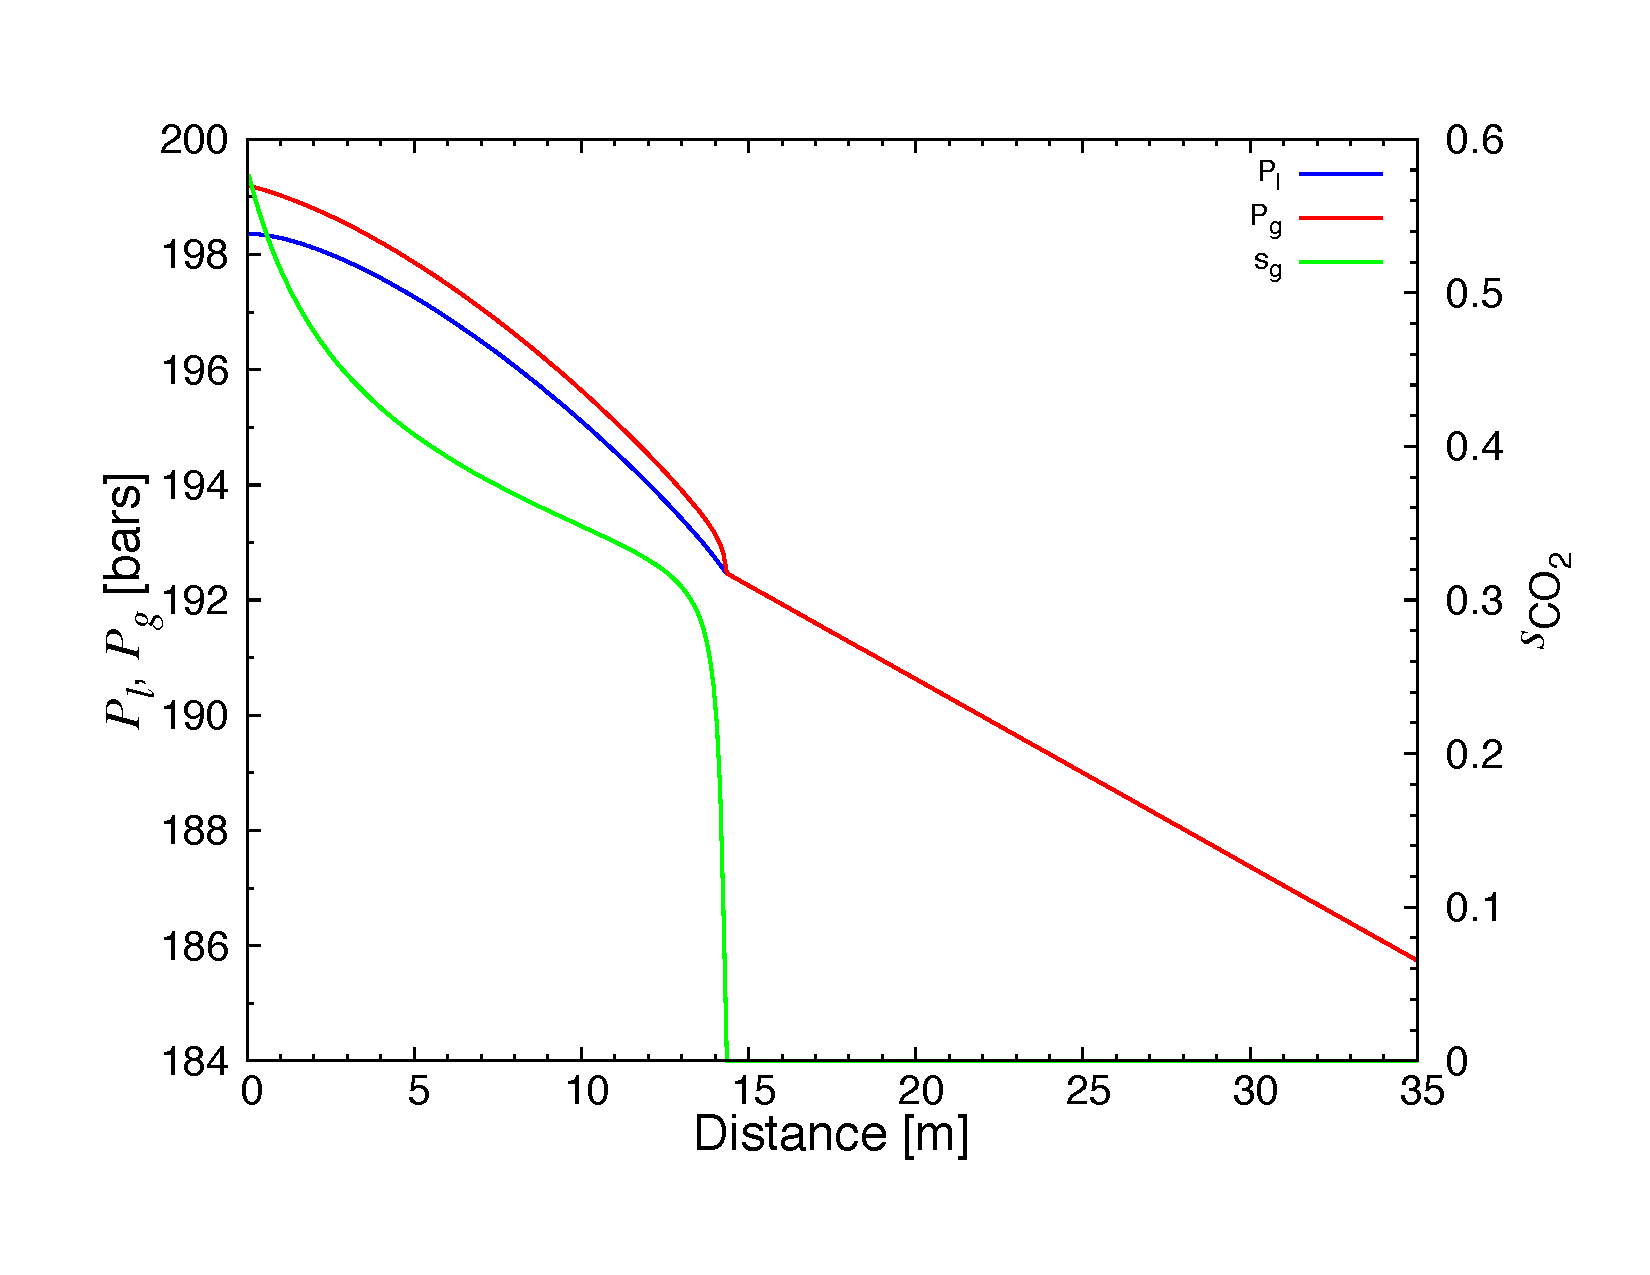
\includegraphics[width=\textwidth]{./figs/p}

\vspace{-1.cm}

\parbox{5in}{
\caption{Liquid (blue curve) and supercritical CO$_2$ (red curve) pressures predicted by PFLOTRAN after an elapsed time of 0.4 y corresponding to the end of injection. Also shown is the CO$_2$ saturation (green curve).}
\label{fp}}
\end{figure}


\clearpage

\subsubsection{CO$_2$ Sequestration in the Presence of a Leaky Well}

The simulation domain has a lateral extent of $1,000\times 1,000$ m and vertical height of 160 m. 
The leaky well is at the center of the domain and the injection well is 100 m east. There are two aquifers at the top and bottom of the domain, each 30 m thick, and an aquitard with thickness of 100 m sandwiched between the two aquifers. 
The leaky well is modeled as a porous medium with a higher permeability compared to the formation. Parameter values used in the simulation are listed in Table~\ref{tleaky_params}. Other parameters used for characteristic curves, heat conduction, etc. may be found in the input file listing (see Table~\ref{tleaky-co2in}).

The initial conditions consist of hydrostatic pressure, and isothermal temperature of 34\degc. The initial pressure at the bottom of the domain is $3.086\times 10^7$ Pa (at 3,000 m depth). 
At the lateral boundaries, hydrostatic boundary conditions are imposed on the system. 
The boundaries at the top and bottom of the domain are no flow boundary conditions. CO$_2$ is injected at a constant rate of 8.87 kg/s for the duration of the simulation of 1000 days and at a constant temperature of 33.6\degc. 

The computational domain was discretized into $200 \!\times\! 200 \!\times\! 32$ grid blocks with spacing $\Delta x \!=\! \Delta y \!=\! 5$ m, and $\Delta z \!=\! 5$ m. The total number of degrees of freedom are 3,840,000. The problem was run on 512 processes on the supercomputer Yellowstone at the NCAR-Wyoming Supercomputing Center.

\begin{table}[h]\centering
\caption{Model parameters.}\label{tleaky_params}

\vspace{3mm}

\begin{tabular}{lccc}
\toprule
Unit & Permeability [m$^2$] & Porosity [---] & Depth [m]\\
\midrule
Aquifer  & $2 \times 10^{-14}$ & 0.15 & 0--30, 130--160  \\ 
Aquitard  & $1\times 10^{-18}$ & 0.15 & 30--130\\
Leaky well  & $1 \times 10^{-12}$ & 0.15 & 0--160\\
\bottomrule
\end{tabular}
\end{table}

Results of the simulation for an elapsed time of 250 days are shown in Figure~\ref{f250d} for liquid pressure and saturation of supercritical CO$_2$. Supercritical CO$_2$ proceeds up the leaky well until it ponds at the top of the domain where a closed boundary is imposed.

The leakage of CO$_2$ through the leaky well as a function of time is shown in Figure \ref{fleaky_flx}. This is defined as the CO$_2$ mass flow midway between the top and bottom domain divided by the injection rate. The maximum value in the leak  occurs at approximately 800 d. The leak begins at approximately 50 d. The results can be compared to Ebigo et al. (2007), Figure 8. It should be noted that the leakage rate is highly sensitive to the lateral grid spacing.
%The maximum leakage value and the leakage value at t = 1,000 days.

\begin{figure}[h]\centering
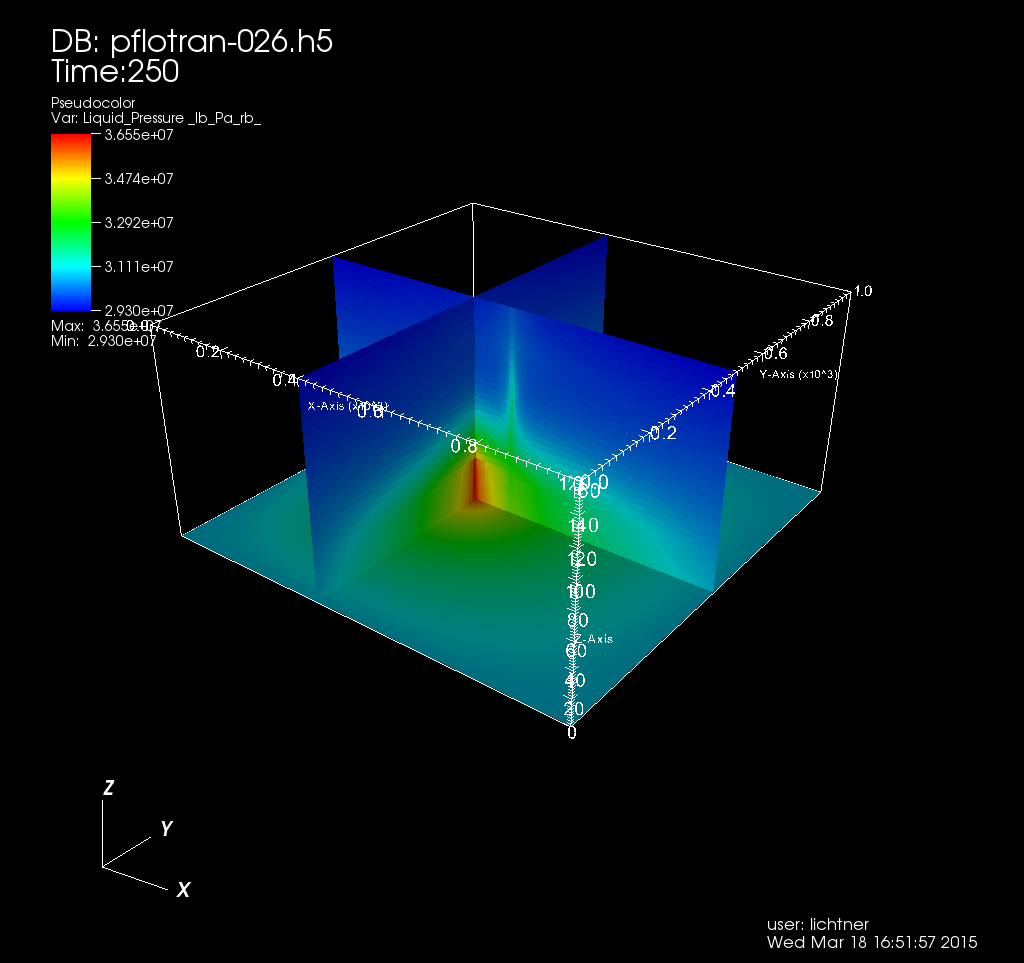
\includegraphics[scale=0.2125]{./figs/liq_p_250d.png}
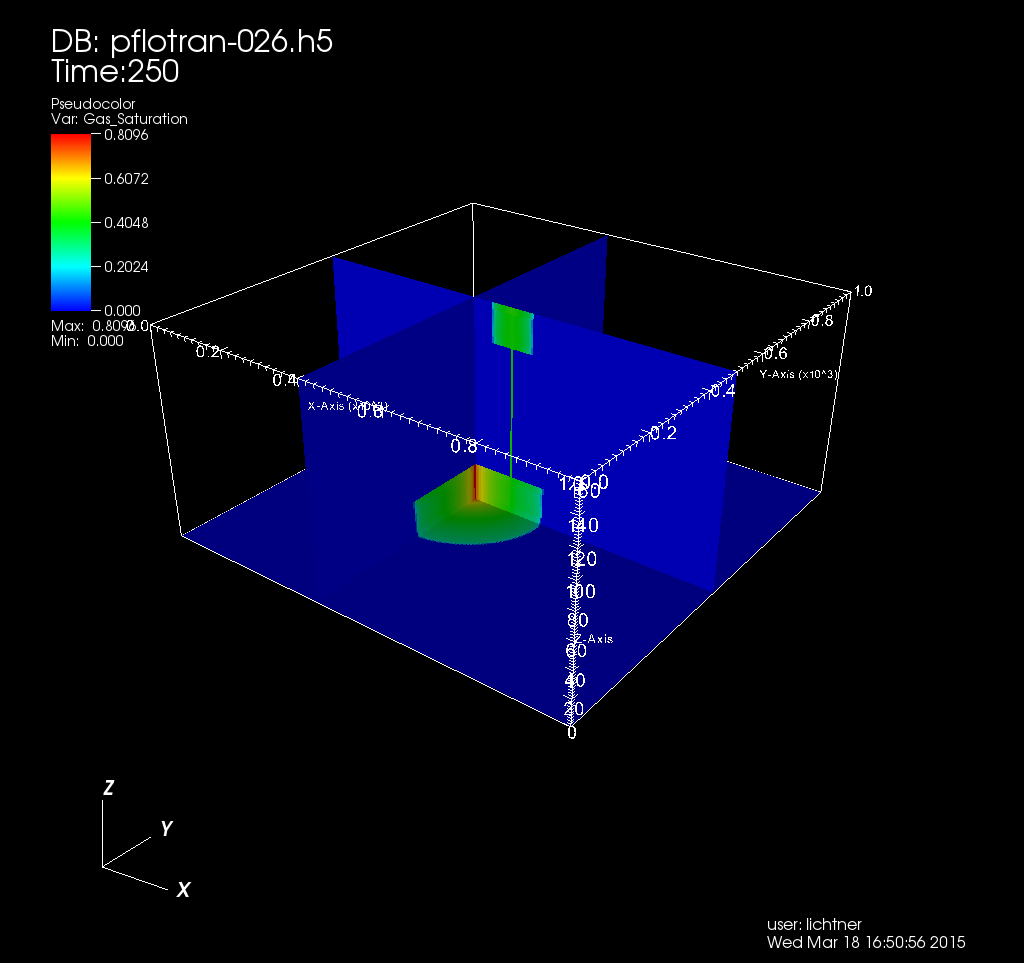
\includegraphics[scale=0.2125]{./figs/sg-250d.png}
\caption{Left: pressure; right: supercritical CO$_2$ saturation; for an elapsed time of 250 days.}\label{f250d}
\end{figure}

\begin{figure}[h]\centering
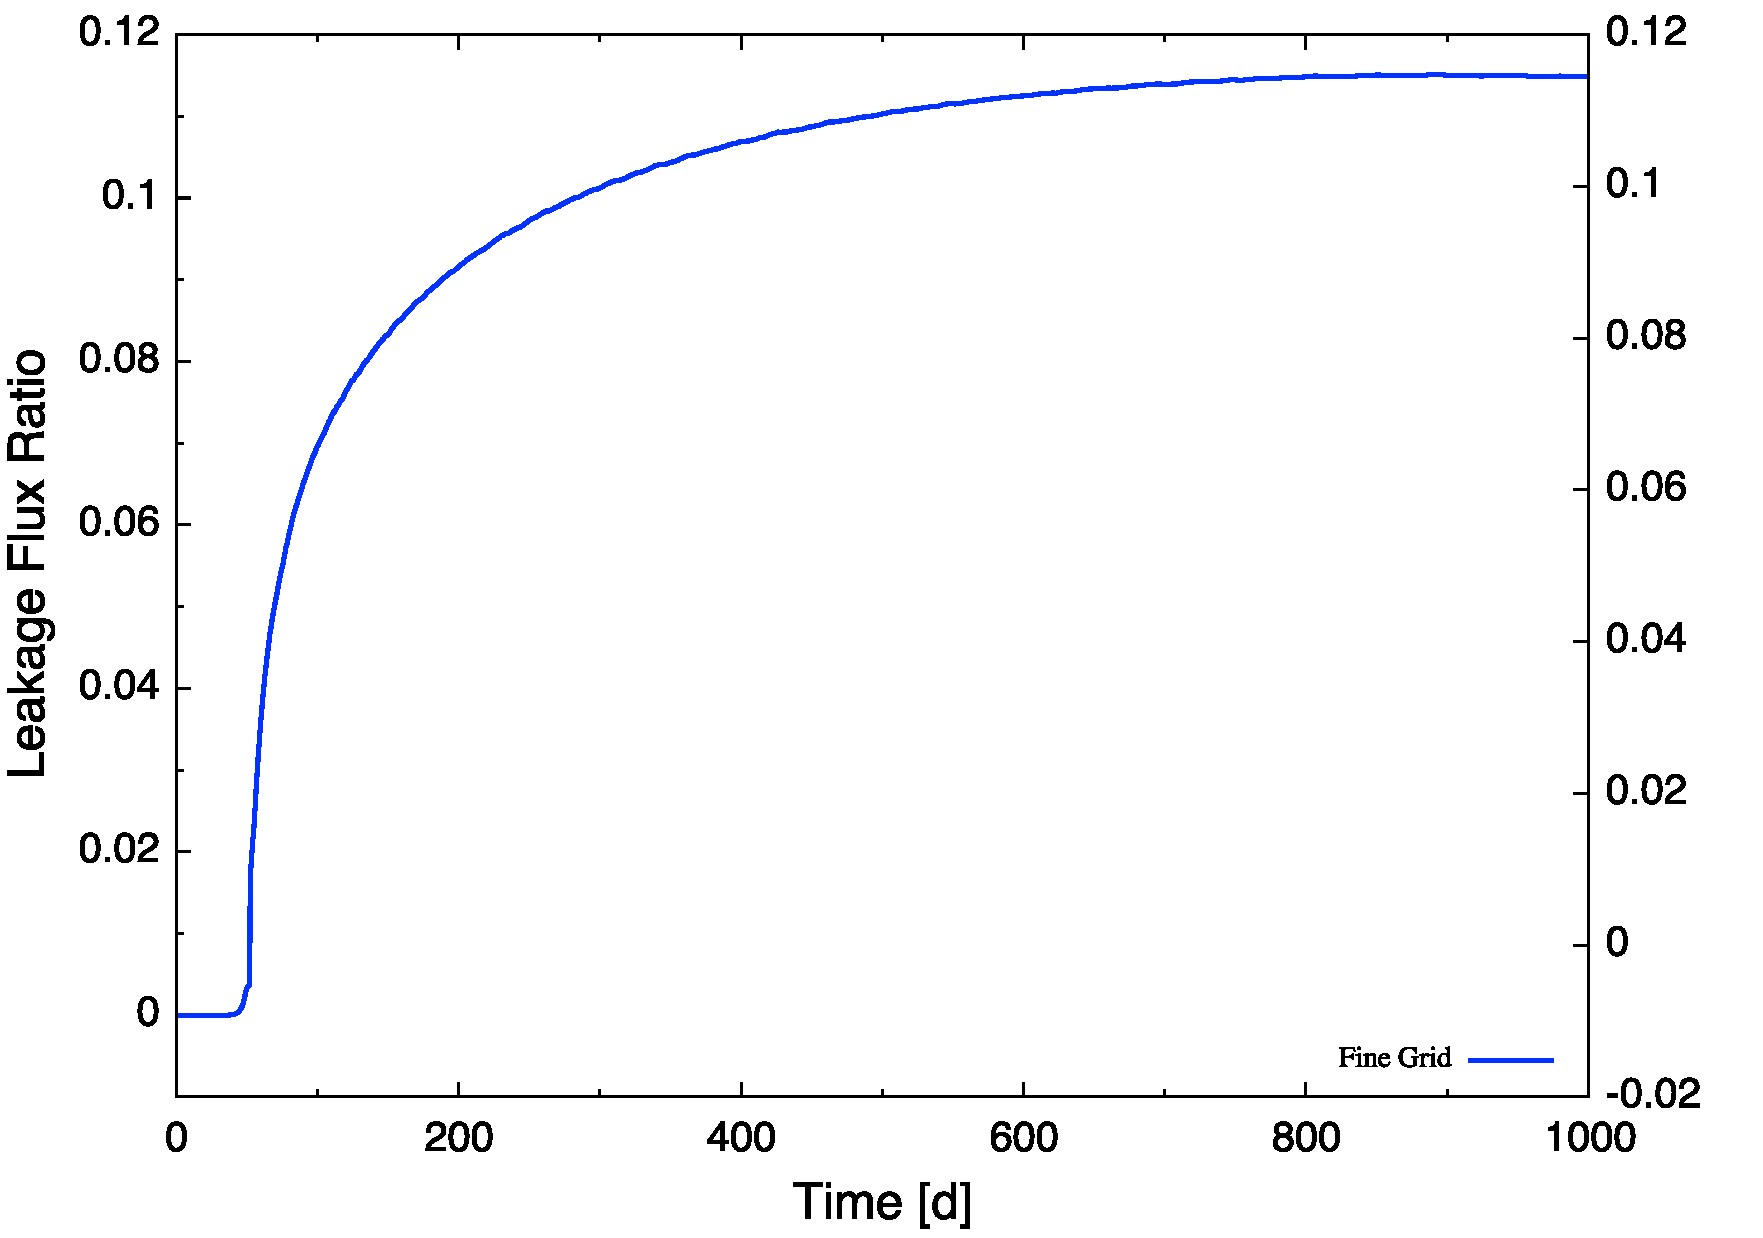
\includegraphics[scale=0.35]{./figs/leakage_flx}
\caption{Leakage rate relative to injection rate.}\label{fleaky_flx}
\end{figure}

\clearpage

\begin{table}[h]
\caption{Input file for 3D CO$_2$ sequestration example problem with a leaky well.}
\end{table}
%\footnotesize
\scriptsize
\VerbatimInput{./inputfiles/CO2/leaky-co2-3d.in}\label{tleaky-co2in}
\normalsize

\newpage
